\documentclass[11pt,compress,t,notes=noshow, aspectratio=169, xcolor=table]{beamer}

\usepackage{../../style/lmu-lecture}
% Defines macros and environments
% This file is included in slides and exercises

% Rarely used fontstyle for R packages, used only in 
% - forests/slides-forests-benchmark.tex
% - exercises/single-exercises/methods_l_1.Rnw
% - slides/cart/attic/slides_extra_trees.Rnw
\newcommand{\pkg}[1]{{\fontseries{b}\selectfont #1}}

% Spacing helpers, used often (mostly in exercises for \dlz)
\newcommand{\lz}{\vspace{0.5cm}} % vertical space (used often in slides)
\newcommand{\dlz}{\vspace{1cm}}  % double vertical space (used often in exercises, never in slides)
\newcommand{\oneliner}[1] % Oneliner for important statements, used e.g. in iml, algods
{\begin{block}{}\begin{center}\begin{Large}#1\end{Large}\end{center}\end{block}}

% Don't know if this is used or needed, remove?
% textcolor that works in mathmode
% https://tex.stackexchange.com/a/261480
% Used e.g. in forests/slides-forests-bagging.tex
% [...] \textcolor{blue}{\tfrac{1}{M}\sum^M_{m} [...]
% \makeatletter
% \renewcommand*{\@textcolor}[3]{%
%   \protect\leavevmode
%   \begingroup
%     \color#1{#2}#3%
%   \endgroup
% }
% \makeatother


\title{Interpretable Machine Learning}
% \author{LMU}
%\institute{\href{https://compstat-lmu.github.io/lecture_iml/}{compstat-lmu.github.io/lecture\_iml}}
\date{}

\begin{document}

% Set style/preamble.Rnw as parent.
\newcommand{\vertiii}[1]{{\left\vert\kern-0.25ex\left\vert\kern-0.25ex\left\vert #1 
    \right\vert\kern-0.25ex\right\vert\kern-0.25ex\right\vert}}
% Load all R packages and set up knitr

% This file loads R packages, configures knitr options and sets preamble.Rnw as 
% parent file
% IF YOU MODIFY THIS, PLZ ALSO MODIFY setup.Rmd ACCORDINGLY...

% Defines macros and environments
 \newcommand{\titlefigure}{figure/AEturtle.jpg}
\newcommand{\learninggoals}{
\item Understand the definition of AEs and their relation to Counterfactual Explanations
\item Understand different methods that generate AEs
\item Discuss potential causes of AEs and standard defenses against them}

\lecturechapter{\Large{Local Explanations: Adversarial Examples}}
\lecture{Interpretable Machine Learning}

% ------------------------------------------------------------------------------

\begin{vbframe}{Adversarial Machine Learning}
Computer systems must be \textbf{robust} i.e. they have to be able to cope with errors or erroneous inputs during execution.
\begin{itemize}
\item \textbf{Adversarial ML} studies the robustness of machine learning (ML) algorithms to malicious input.
\item We differentiate between two different kinds of attacks: evasion and poisoning.
\item \textbf{Evasion attacks} mislead an employed ML model with manipulated inputs. We focus on these in this lecture.
\item In \textbf{poisoning}, an attacker enters malicious inputs to the training dataset. This weak spot can be exploited by the attacker after model training, e.g., the attacker can trigger a specific behavior of the model for a specific input. 
%\item \textbf{Model Stealing} encompass methods by which an attacker can recover a model or the data it was trained on.
\end{itemize}
\end{vbframe}

\begin{vbframe}{Adversarial Examples}
%The inputs by which evasion attacks can be conducted are called \textbf{Adversarial Examples (AEs)}
\begin{itemize}
\item An AE is an input to a model that is deliberately designed to "fool" the model into misclassifying it.
\item AEs occur even for ML algorithms with low generalization error on a test set.
\item Deep Learning (DL) algorithms like Convolutional Neural Networks (CNNs) are particularly vulnerable to such attacks, but classical ML models are often, too.
\item AEs that are created from a real data instance $\xv$ are often indistinguishable from $\xv$ by a human observer. Such cases suggest that even models with a very good test set performance have no deep understanding of the underlying concepts.% that determine the correct output label.
\end{itemize}
\end{vbframe}

\begin{vbframe}{Examples: Model-Attacks}
\begin{figure}[h]
\centering
  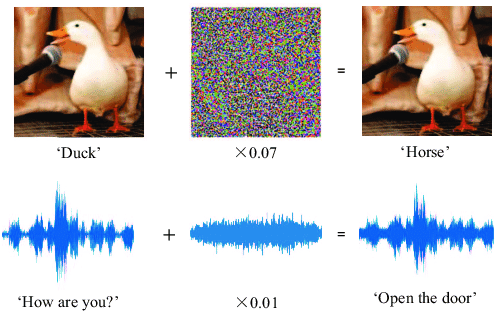
\includegraphics[width=0.6\linewidth]{figure/AEduckSound.png}
  \caption{On the left side, we see real instances of image and audio data  correctly classified. The middle column, depicts a noisy input in the same spaces. Column three shows the summation of the original inputs plus the noisy input multiplied by a small scalar. The resulting data points are AEs as they get the wrong label assigned.}
  \label{fig:mnist}
\end{figure} 

\footnote[frame]{Gong \& Poellabauer (2018). An Overview of Vulnerabilities of Voice Controlled Systems. https://arxiv.org/pdf/1803.09156.pdf.}


%eykholt stop sign
%brown turtle
%Gong duck and sound
%@inproceedings{inproceedings,
%author = {Gong, Yuan and Poellabauer, Christian},
%year = {2018},
%month = {03},
%pages = {},
%title = {An Overview of Vulnerabilities of Voice Controlled Systems}
%}
\end{vbframe}

\begin{vbframe}{Examples: Image Data}
\begin{figure}[h]
\centering
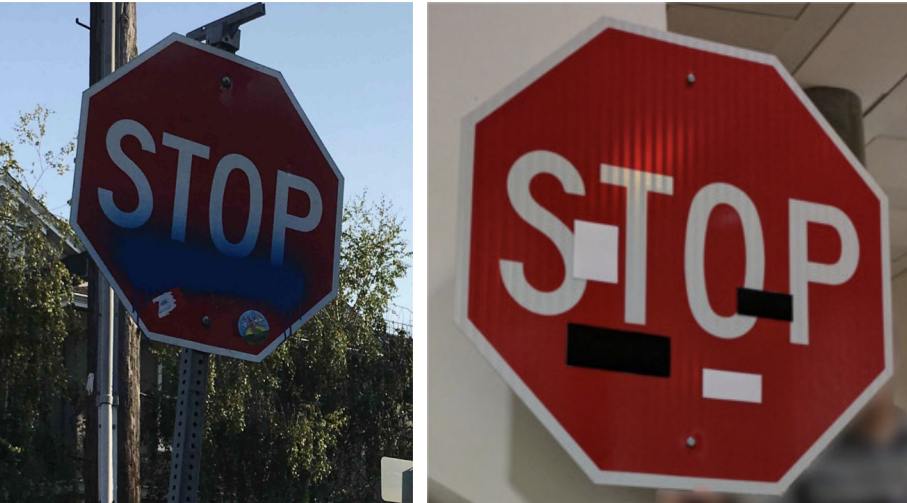
\includegraphics[width=0.46\linewidth]{figure/AEstop.png}\quad 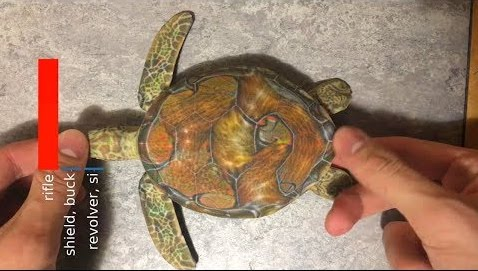
\includegraphics[width=0.45\linewidth]{figure/AEturtle.jpg}
  \caption{The images show AEs employed in a real-world application. The stop sign on the right is an input designed to resemble a normal stop sign with graffiti on it like the one on the left. It is misclassified as a right of way sign. On the right image, we see a 3D-print turtle. It is designed in a way that it is misclassified as a rifle from every angle of presentation.} 
  \label{fig:mnist}
\end{figure} 

\footnote[frame]{Eykholt et al. (2018). Physical Adversarial Examples for Object Detectors. https://arxiv.org/pdf/1807.07769.pdf.} 
\footnote[frame]{Athalye et al. (2018). Synthesizing Robust Adversarial Examples. https://arxiv.org/pdf/1707.07397.pdf. \href{https://www.youtube.com/watch?v=piYnd_wYlT8}{Link to video.}}

%eykholt stop sign
%brown turtle
%Gong duck and sound
%@inproceedings{inproceedings,
%author = {Gong, Yuan and Poellabauer, Christian},
%year = {2018},
%month = {03},
%pages = {},
%title = {An Overview of Vulnerabilities of Voice Controlled Systems}
%}
\end{vbframe}

\begin{vbframe}{Example: Tabular Data}
For tabular data, it is difficult to define imperceptibility properly.% Expert knowledge is required in evaluation.
\begin{itemize}
    \item Idea: experts focus on the most important features in their judgment.
%    \item Tabular features have specific natural ranges that must be respected.
    \item An AE arises from manipulating features the model deems important but experts do not.
\end{itemize}
\begin{figure}[h]
\centering
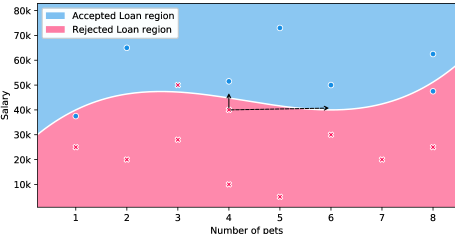
\includegraphics[width=0.6\linewidth]{figure/AEloanApplication.png}
  \caption{The image depicts the decision boundary of a classifier that decides about loan applications. Number of pets should not influence loan acceptance.}
  \label{fig:mnist}
\end{figure} 
\vspace{-0.75cm}
\footnote[frame]{Ballet (2019). Imperceptible Adversarial Attacks on Tabular Data. https://arxiv.org/pdf/1911.03274.pdf}

\end{vbframe}

\begin{vbframe}{AEs and Interpretability}
From the examples, we can see that AEs pose security threats to the use of ML algorithms in real world applications. But what is their connection to interpretability?

\begin{itemize}
    \item AEs show where models fail and can therefore increase the understanding of the model.
    \item AEs motivate the need for interpretability.
    \item Interpretation techniques can provide insights into how to improve ML algorithms and make them more robust against AEs.
    \item Explanations to end users may enclose too much information about the used model. This information can be used to construct adversarial attacks.
\end{itemize}
\end{vbframe}

\begin{vbframe}{Formal Definition}
\begin{block}{Adversarial Input}
Let $\epsilon>0$, $f:\Xspace \rightarrow \Yspace$ be an ML model, $y'\in \Yspace$ be a desired output, and $\xv \in \Xspace$ be a real data point that is correctly classified: $f(\xv)=y_{\xv,true}$. \\ 
 We call $a_{\xv}$ an \textbf{adversarial input} to $\xv$ if:
\begin{equation*}
    \| a_{\xv}- \xv\|<\epsilon\text{ and } f(a_{\xv})\neq y_{a_{\xv},true}=f(\xv).
\end{equation*}
Moreover, we call $a_{\xv}$ \textbf{targeted} if $f(a_{\xv})=y'$.
\end{block}
\begin{itemize}
    \item Intuitively speaking an adversarial is a data point close to a real, correctly classified input that is misclassified.
    \item It is called targeted if the class it is assigned to is determined.
%    \item An AE is the depiction of such an input in visual, textual or any other form. 
    \item The above definition of adversarials is restricted to classification tasks but it can be generalized to regression problems.
\end{itemize}
\end{vbframe}


\begin{vbframe}{AEs and Counterfactual Explanations}
It seems as if AEs and counterfactual explanations (CEs) are defined similarly. Both AEs and CEs describe inputs close to a given input $\xv$ that gets a different assignment. What are their differences?
\begin{itemize}
    \item Counterfactuals do not have to be misclassified.
%    \item Counterfactuals should be maximally close to $\xv$.
    \item Different notions of distance $\|\cdot\|$ are applied, e.g., $p_{2,\infty}$-norm for AEs or $p_{0,1}$-norm for CEs.
    \item Informal difference I: AEs are mostly considered for high-dimensional data, while CEs are mostly considered in the context of low-dimensional data.
    \item Informal difference II: AEs hide changes while CEs highlight them.
    \item \textbf{Shared example:} ``If you had two more pets, your loan application would have been granted" is an example of both AEs and CEs.
\end{itemize}
\end{vbframe}

\begin{vbframe}{Why Do AEs Exist?}
In the following, we present a non-exhaustive list of hypotheses:
\begin{itemize}
    \item \textbf{Low-Probability Spaces Hypotheses:} AEs live in low-probability yet dense spaces in the data manifold that are not well represented in the training samples.
    %@article{szegedy2013intriguing,
 % title={Intriguing properties of neural networks},
 % author={Szegedy, Christian and Zaremba, Wojciech and Sutskever, Ilya and Bruna, Joan and Erhan, Dumitru and Goodfellow, Ian and Fergus, Rob},
 % journal={arXiv preprint arXiv:1312.6199},
 % year={2013}
%}
    \item \textbf{Linearity Hypotheses (most popular):} Adversarial examples are omnipresent in the data manifold. They occur, because commonly used models often show linear behavior. Small changes of $\epsilon$ in every feature cause a change of $\epsilon\|\thetab\|_1$ in prediction ($\thetab$ are the weights in the linear function).
    %@article{goodfellow2014explaining,
 % title={Explaining and harnessing adversarial examples},
 % author={Goodfellow, Ian J and Shlens, Jonathon and Szegedy, Christian},
 % journal={arXiv preprint arXiv:1412.6572},
 % year={2014}
%}
    \item \textbf{The Boundary Tilting Hypothesis:} Linearity is neither necessary nor sufficient to explain AEs. Instead, AEs mostly result from overfitting the sampled manifold.
 %   @article{tanay2016boundary,
 % title={A boundary tilting perspective on the phenomenon of adversarial examples},
 % author={Tanay, Thomas and Griffin, Lewis},
 % journal={arXiv preprint arXiv:1608.07690},
 % year={2016}
%}
    \item \textbf{Human-Centric Hypotheses:} ML models make use of predictive but non-robust features. These are features that are highly correlated with the prediction target, but not used by humans.
    %cite: @article{ilyas2019adversarial,
%  title={Adversarial Examples Are Not Bugs, They Are Features},
%  author={Ilyas, Andrew and Santurkar, Shibani and Engstrom, Logan and Tran, Brandon and Madry, Aleksander},
%  journal={Advances in neural information processing systems},
%  volume={32},
%  year={2019}
%}
\end{itemize}
\vspace{-0.2cm}
\footnote[frame]{(1) Szegedy et al. (2013). Intriguing properties of neural networks; (2) Goodfellow et al. (2014). Explaining and harnessing adversarial examples; (3) Tanay and Griffin (2016). A boundary tilting perspective on the phenomenon of adversarial examples; (4) Ilyas et al. (2019). Adversarial Examples Are Not Bugs, They Are Features. Advances in neural information processing systems.}
\end{vbframe}

\begin{vbframe}{Ways to Generate AEs}
There exist various ways in the literature to generate AEs for a given model in feasible time. We can...
\begin{itemize}
    \item formulate the search for AEs as an \textbf{optimization problem}, e.g. 
    \begin{equation*}
        \label{eq:optimization}
        \underset{\xv'\in \Xspace}{\text{argmin}}\; \| \xv-\xv' \|_{\Xspace}+\lambda\;    \|f(\xv')-y'\|_{\Yspace}.
    \end{equation*}
    \item use \textbf{sensitivity analysis} to identify features that influence the target class.
    \item train a generative network to generate adversarials.
\end{itemize}
Moreover, depending on the attacker's model access, we can distinguish between...
\begin{itemize}
    \item \textbf{Full-access attacks}: the attacker has full access to the internals of the model.
    \item \textbf{Black-box attacks}: the attacker can only query the model on some inputs and receives the model's outputs.
\end{itemize}
\end{vbframe}

\begin{vbframe}{Fast-Gradient-Sign-Method (FGSM)}
Since we have seen optimization methods for CEs, we focus on a method using sensitivity analysis, namely FGSM.
\begin{itemize}
    \item FGSM is based on the linearity hypothesis.
    \item FGSM finds AEs from:
    \begin{equation*}
        a_{\xv}=\xv+\epsilon\cdot\text{sign}(\nabla_{\xv} J(\theta,\xv,y_{\xv,true}))
    \end{equation*}
    where $\text{sign}(\nabla_{\xv} J(\theta,x,y_{\xv,true}))$ describes the component-wise signum of the Gradient of cost function $J$ in $\xv$ with true label $y_{\xv,true}$.
\end{itemize}
\begin{figure}[h]
\centering
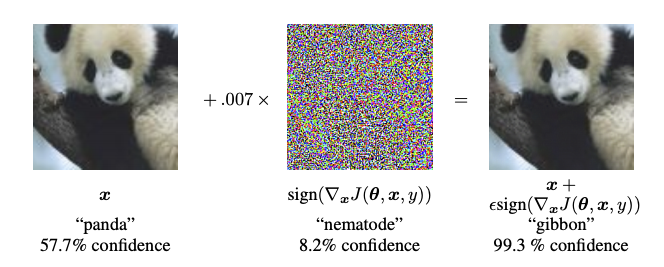
\includegraphics[width=0.5\linewidth]{figure/AEpanda.png}
  \caption{An AE generated with the FGSM.}
  \label{fig:mnist}
\end{figure} 
\vspace{-0.6cm}
\footnote[frame]{Goodfellow et al. (2015). Explaining and Harnessing Adversarial Examples. https://arxiv.org/pdf/1412.6572.pdf.}
\end{vbframe}

\begin{vbframe}{Fast-Gradient-Sign-Method (FGSM)}
\begin{itemize}
    \item FGSM works particularly well for linear(-like) models in high-dimensional spaces, e.g., LSTMs, logistic regressions or CNNs with ReLU activations.
    \item Not every $a_{\xv}$ generated by FGSM is an AE, especially if $\epsilon$ is too small.
    \item FGSM attacks can be also generated without model access by approximating the gradient, i.e. with finite difference methods.
    \item The notion of similarity in FGSM is based on $\|\cdot\|_{\infty}$. However, there exist generalizations of FGSM to other norms.
\end{itemize}
%@inproceedings{lyu2015unified,
%  title={A unified gradient regularization family for adversarial examples},
%  author={Lyu, Chunchuan and Huang, Kaizhu and Liang, Hai-Ning},
%  booktitle={2015 IEEE international conference on data mining},
%  pages={301--309},
%  year={2015},
%  organization={IEEE}
%}
\end{vbframe}


\begin{vbframe}{Black-Box Attacks with Surrogates}
The biggest threat comes from AEs that can be generated in a black-box scenario. Among these, approaches based on surrogates are conceptually most interesting.
\begin{itemize}
    \item Query the model you aim to attack as often as allowed on data similar to the training data.
    \item Use the labeled data you received to train a surrogate model.% by supervised learning e.g. a CNN.
    \item %Use white-box methods (e.g. Gradient-Based-Methods) to g
    Generate AEs for the surrogate model.% for the given optimisation problem.
    \item Use these AEs to attack the original model.
\end{itemize}
Several experiments showed that such attacks are often successful. % Papernot et al. call 
This phenomenon is known as the \textbf{transferability} of AEs.
%
%
%@article{papernot2016transferability,
  %title={Transferability in machine learning: from phenomena to %black-box attacks using adversarial samples},
  %author={Papernot, Nicolas and McDaniel, Patrick and Goodfellow,
  %Ian},
%  journal={arXiv preprint arXiv:1605.07277},
%  year={2016}
%}
\footnote[frame]{Papernot et al. (2016). Transferability in machine learning: from phenomena to black-box attacks using adversarial samples.}
\end{vbframe}

\begin{vbframe}{Defenses Against AEs}
There are several ways to protect your network against such attacks. We distinguish between two broad types of defenses, differing in the position in which they act.
\begin{itemize}
    \item \textbf{Guards} act on the inputs a model receives. They include methods to \textbf{detect anomalies} (e.g., statistical testing, or discriminator networks from GANs), or to \textbf{conduct transformations} on inputs (e.g. PCA).
    \item \textbf{Defense by design} act on the employed model itself. It includes methods like \textbf{adversarial training} (train model on adversarials) or \textbf{architectural defenses} (e.g., removing low predictive features from the model) % or imposing layer-wise constraints on the output variance) 
    to make models more robust against AEs.
\end{itemize}
\end{vbframe}

%\begin{vbframe}{Regularization Against AEs}
%The use of regularization techniques against AEs is motivated by most hypotheses that explain AEs. As an example we look at a technique based on the FGSM and the linearity hypotheses.
%\begin{itemize}
%    \item Goodfellow et al. suggest to specfiy the cost function s.t.
%    \begin{equation*}
%        \tilde{J}(\theta,\xv,y):=\alpha J(\theta,\xv,y)+(1-\alpha) J(\theta,\xv+\epsilon\cdot\text{sign}(\nabla_{\xv} J(\theta,\xv,y)),y)
%    \end{equation*}
%    with $\alpha=0.5$.
%    \item This increased the model robustness against FGSM generated AEs.
%    \item However, model are not only still prone to other AEs but also to many FGSM-AEs.
%    \item Applying such regularization terms can increase test error.
%\end{itemize}
%\end{vbframe}

\begin{vbframe}{Summary}
\begin{itemize}
    \item AEs are not explanations themselves but are conceptually connected to them.
    \item AEs can be generated in diverse settings. Crucial modeling decisions are the distance measure, the local environment, and the target level (model or process).
    \item There are various hypotheses on the existence of AEs which also motivate different defense strategies.
\end{itemize}
\end{vbframe}

%\begin{vbframe}{Outlook}
%\begin{itemize}
%    \item Even in highly non-linear models AEs occur. As long as their existence is not well-understood, defenses against them will have limited power.
%    \item More and more different distance measures are considered, e.g. $p_0$ for one-pixel attacks, the Wasserstein-metric or psychologically motivated measures like the Perceptual Adversarial Similarity Score (PASS).
%    \item Recent work considered AEs that fool both, humans and ML models. AEs may be a case where research on human and machine perception can profit from each other.
%\end{itemize}
%@misc{rozsa2016adversarial,
%      title={Adversarial Diversity and Hard Positive Generation}, 
%      author={Andras Rozsa and Ethan M. Rudd and Terrance E. Boult},
%      year={2016},
%      eprint={1605.01775},
%      archivePrefix={arXiv},
%      primaryClass={cs.CV}
%}
%\end{vbframe}

\begin{vbframe}{Central References}
\begin{itemize}
    \item Serban, A., Poll, E., \& Visser, J. (2020). Adversarial examples on object recognition: A comprehensive survey. ACM Computing Surveys (CSUR), 53(3), 1-38.
    \item Goodfellow, I. J., Shlens, J., \& Szegedy, C. (2014). Explaining and harnessing adversarial examples. arXiv preprint arXiv:1412.6572.
    \item Yuan, X., He, P., Zhu, Q., \& Li, X. (2019). Adversarial examples: Attacks and defenses for deep learning. IEEE transactions on neural networks and learning systems, 30(9), 2805-2824.
\end{itemize}
\end{vbframe}


\endlecture
\end{document}
